\documentclass[a4paper,oneside,12pt]{report}
\usepackage{fontspec}
\usepackage{setspace}
\usepackage{graphicx}
\usepackage{titling}
\usepackage{geometry}
\usepackage{listings}
\usepackage{xcolor}
\usepackage{float}
\usepackage{hyperref}
\usepackage{indentfirst}
\usepackage{url}
\usepackage{fancyhdr}
\usepackage{tocloft}
\usepackage{bookmark}
\usepackage{booktabs}
\usepackage{caption}

\setmainfont{TeX Gyre Termes}
\onehalfspacing
\geometry{left=3cm, right=2.5cm, top=2cm, bottom=2.5cm}
\sloppy

\definecolor{codegreen}{rgb}{0,0.6,0}
\definecolor{codegray}{rgb}{0.5,0.5,0.5}
\definecolor{codepurple}{rgb}{0.58,0,0.82}
\definecolor{backcolour}{rgb}{0.95,0.95,0.92}
\definecolor{darkblue}{rgb}{0,0,0.6}

\lstdefinestyle{commonstyle}{
    backgroundcolor=\color{backcolour},
    breakatwhitespace=false,
    breaklines=true,
    captionpos=b,
    keepspaces=true,
    numbers=left,
    numbersep=5pt,
    showspaces=false,
    showstringspaces=false,
    showtabs=false,
    tabsize=2,
    frame=single,
    basicstyle=\ttfamily\footnotesize,
    numberstyle=\tiny\color{codegray},
    columns=flexible,
    postbreak=\mbox{\textcolor{red}{$\hookrightarrow$}\space},
    breakindent=0pt,
    breakautoindent=false
}
\lstdefinestyle{bashstyle}{
    style=commonstyle,
    language=bash,
    commentstyle=\color{codegreen},
    keywordstyle=\color{darkblue},
    stringstyle=\color{codepurple}
}
\lstdefinestyle{yamlstyle}{
    style=commonstyle,
    commentstyle=\color{codegreen},
    keywordstyle=\color{darkblue},
    stringstyle=\color{codepurple}
}

\newcommand{\customfbox}[1]{%
  \setlength{\fboxsep}{0pt}%
  \setlength{\fboxrule}{0.5pt}%
  \fcolorbox{black}{white}{#1}%
}
\renewcommand{\figurename}{Gambar}
\renewcommand{\thefigure}{\arabic{figure}}
\hypersetup{
    colorlinks=true,
    linkcolor=black,
    filecolor=black,
    urlcolor=black,
    citecolor=black,
    pdftitle={Laporan KEPL Pertemuan 3},
    pdfpagemode=FullScreen,
    breaklinks=true
}
\pagestyle{fancy}
\fancyhf{}
\fancyfoot[C]{\thepage}
\renewcommand{\headrulewidth}{0pt}
\fancypagestyle{plain}{
    \fancyhf{}
    \fancyfoot[C]{\thepage}
    \renewcommand{\headrulewidth}{0pt}
}
\renewcommand{\contentsname}{Daftar Isi}
\renewcommand{\bibname}{Daftar Pustaka}
\renewcommand{\thechapter}{}
\renewcommand{\chaptername}{}
\renewcommand{\thesection}{\arabic{chapter}.\arabic{section}}
\renewcommand{\thesubsection}{\thesection.\arabic{subsection}}
\setcounter{secnumdepth}{3}
\setcounter{tocdepth}{3}
\renewcommand{\cftchapdotsep}{\cftdotsep}
\renewcommand{\cftchapleader}{\cftdotfill{\cftchapdotsep}}
\setlength{\cftchapindent}{0em}
\setlength{\cftsecindent}{2em}
\setlength{\cftsubsecindent}{4em}
\setlength{\cftchapnumwidth}{0em}
\setlength{\cftsecnumwidth}{2.5em}
\setlength{\cftsubsecnumwidth}{3.2em}
\renewcommand{\cftchappresnum}{}
\renewcommand{\cftchapaftersnum}{}
\newcommand{\tocboldsection}[1]{%
  \protect\renewcommand{\protect\cftchapfont}{\protect\bfseries}%
  #1%
  \protect\renewcommand{\protect\cftchapfont}{}%
}

\begin{document}

\newgeometry{left=3cm, right=2.5cm, top=2.5cm, bottom=3cm}
\begin{titlingpage}
\begin{spacing}{1}
\begin{center}
\vspace*{0.2cm}
{\large \textbf{\MakeUppercase{Laporan Praktikum}}} \\[0.4cm]
{\large \textbf{\MakeUppercase{Konstruksi dan Evolusi Perangkat Lunak}}} \\[0.4cm]
{\large \textbf{\MakeUppercase{Pertemuan 3}}} \\[0.4cm]
{\large \textbf{\MakeUppercase{Continuous Deployment untuk Laravel}}} \\[1.5cm]


\includegraphics[height=7cm]{images/UGM.png} \\[0.7cm]

{\normalsize \textbf{Disusun oleh:}} \\[0.4cm]
\begin{tabular}{@{}l l @{}}
  \textbf{Nama}           & : Hafidz Rizqullah Prasetya \\
  \textbf{NIM}            & : 24/535493/SV/24243 \\
  \textbf{Kelas}          & : PL5A1 \\
  \textbf{Dosen Pengampu} & : Galih Malela Damaraji \\
\end{tabular} \\[1.2cm]

{\normalsize \textbf{PROGRAM STUDI D-IV}} \\[0.2cm]
{\normalsize \textbf{TEKNOLOGI REKAYASA PERANGKAT LUNAK}} \\[0.2cm]
{\normalsize \textbf{DEPARTEMEN TEKNIK ELEKTRO DAN INFORMATIKA}} \\[0.2cm]
{\normalsize \textbf{SEKOLAH VOKASI}} \\[0.2cm]
{\normalsize \textbf{UNIVERSITAS GADJAH MADA}} \\[0.2cm]
{\normalsize \textbf{YOGYAKARTA}} \\[0.2cm]
{\normalsize \textbf{2026}} \\[1.2cm]
\end{center}
\end{spacing}
\end{titlingpage}
\restoregeometry

\thispagestyle{empty}
\clearpage
\stepcounter{page}
\thispagestyle{empty}

\addcontentsline{toc}{chapter}{Daftar Isi}
\tableofcontents
\clearpage

\pagenumbering{arabic}
\setcounter{page}{3}

\chapter[Tujuan Praktikum]{Tujuan Praktikum}
Sesuai arahan pada pertemuan ketiga dan deskripsi tugas di Google Classroom \textit{Konstruksi dan Evolusi Perangkat Lunak 2026}, tujuan praktikum ini adalah:
\begin{enumerate}
   \item Mahasiswa mampu menyusun pipeline empat tahap (\texttt{build}, \texttt{test}, \texttt{staging}, \texttt{production}) yang dirangkai dengan \texttt{needs:}.
   \item Mahasiswa mampu menjaga agar tahap deploy hanya berjalan dari branch \texttt{main} dan menunggu persetujuan manusia lewat \textit{environment} dengan \textit{required reviewer}.
   \item Mahasiswa mampu menuliskan urutan langkah deploy Laravel di server sebagai skrip \texttt{deploy.sh} yang berhenti saat ada perintah gagal.
   \item Mahasiswa mampu membuktikan bahwa pipeline benar-benar menghentikan tahap berikutnya ketika satu pengujian sengaja digagalkan.
\end{enumerate}

\clearpage

\chapter{Dasar Teori}

\section{Continuous Deployment dan Perbedaannya dengan Continuous Integration}
Continuous Integration (CI) memverifikasi setiap perubahan secara otomatis, sedangkan Continuous Deployment (CD) melanjutkan langkah itu sampai perubahan benar-benar terpasang di server \cite{fowler-ci,humble2010}. Pertemuan sebelumnya berhenti di tahap CI: kode diuji dan gaya kodenya diperiksa, lalu selesai. Pertemuan ini menambah tahap setelahnya, yaitu \texttt{staging} dan \texttt{production}, sehingga pipeline menyerupai alur rilis yang sebenarnya.

\section{Pipeline Bertahap dengan \texttt{needs:}}
GitHub Actions menjalankan setiap job di mesin yang bersih, sehingga tiap job harus menyiapkan ulang apa yang dibutuhkannya \cite{github-actions}. Kata kunci \texttt{needs:} membuat sebuah job menunggu job lain selesai lebih dulu \cite{github-needs}. Kalau job yang ditunggu gagal, job setelahnya tidak dijalankan sama sekali dan statusnya menjadi \textit{skipped}. Sifat inilah yang dipakai untuk menghentikan deploy ketika pengujian gagal.

\begin{figure}[H]
    \centering
    \customfbox{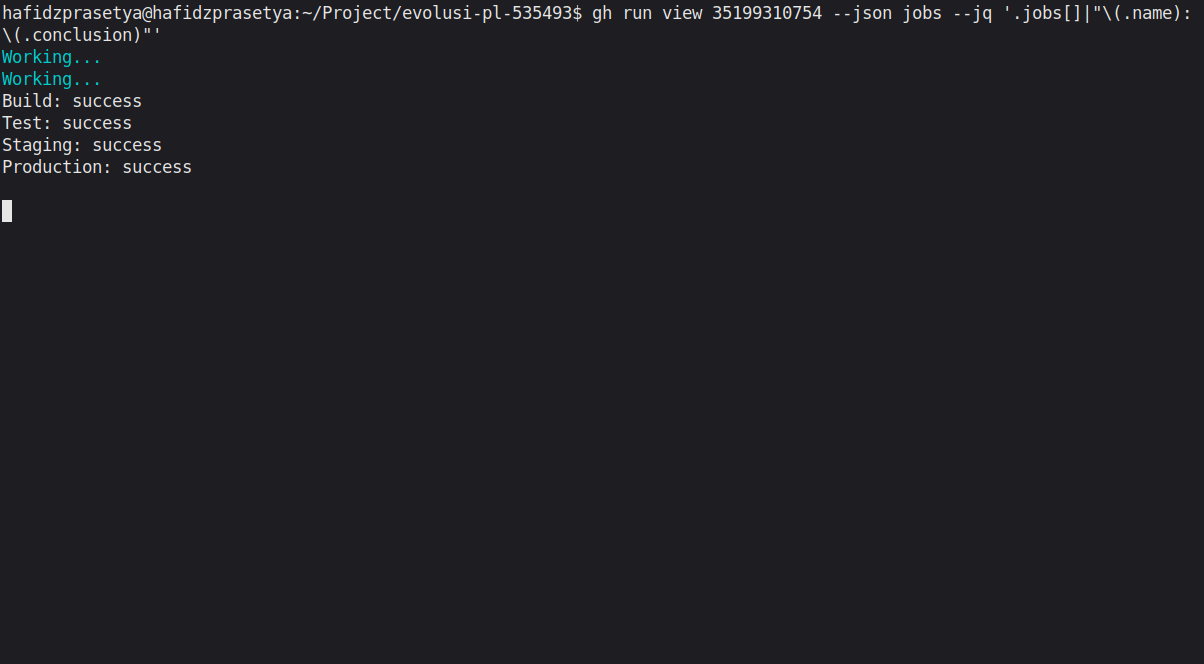
\includegraphics[width=0.95\textwidth]{images/ss-01-empat-job-hijau.png}}
    \caption{Keempat job pipeline (\texttt{Build}, \texttt{Test}, \texttt{Staging}, \texttt{Production}) hijau pada satu run.}
    \label{fig:empat-job}
\end{figure}

\section{Environment dan Required Reviewer}
\textit{Environment} pada GitHub Actions adalah wadah berisi variabel dan aturan perlindungan untuk satu tujuan deploy \cite{github-environments}. Ketika sebuah job memakai \texttt{environment: production} dan environment tersebut punya \textit{required reviewer}, job berhenti di status \textit{waiting} sampai ada orang yang menyetujui. Cara ini membuat deploy ke produksi tidak pernah berjalan sendiri tanpa sepengetahuan pemilik proyek.

\section{Urutan Langkah Deploy Laravel}
Deploy aplikasi Laravel di server mengikuti urutan yang tidak boleh ditukar \cite{laravel-docs}. Aplikasi ditutup dulu dengan \texttt{php artisan down}, kode terbaru ditarik, dependensi produksi dipasang tanpa paket pengembangan, migrasi basis data dijalankan, cache dibangun ulang, pekerja antrean dimuat ulang, lalu aplikasi dibuka kembali dengan \texttt{php artisan up}. Baris \texttt{set -e} di awal skrip penting karena tanpa itu skrip akan terus berjalan walaupun satu perintah gagal, dan aplikasi bisa terbuka dalam keadaan rusak \cite{stauffer2023}.

\section{Artefak Antar Job}
Karena setiap job mulai dari mesin kosong, hasil pekerjaan satu job perlu diteruskan ke job berikutnya. \texttt{actions/upload-artifact} dan \texttt{actions/download-artifact} dipakai untuk memindahkan berkas antar job \cite{github-artifacts}. Pada praktikum ini direktori \texttt{vendor} hasil \texttt{composer install} di job \texttt{build} diunggah sebagai artefak, lalu diunduh oleh job \texttt{test}, sehingga pemasangan dependensi cukup dilakukan sekali.

\clearpage

\chapter[\tocboldsection{Hasil dan Pembahasan}]{Hasil dan Pembahasan}
Pada bab ini saya menjelaskan pekerjaan untuk Tugas 2 sesuai instruksi di Classroom. Saya melanjutkan repository \texttt{evolusi-pl-535493} dari minggu sebelumnya, tidak membuat repository baru. Semua langkah saya verifikasi lewat GitHub Actions dan eksekusi lokal.

\section{Alat dan Bahan}
Alat dan bahan yang digunakan:
\begin{itemize}
    \item Laptop dengan OS Linux, akses internet, dan akun GitHub \texttt{hafidzrizqullahprasetya}.
    \item Git, GitHub CLI (\texttt{gh}), PHP 8.5.10, Composer 2.10.3, Laravel 13, PHPUnit, dan Laravel Pint.
    \item Repository: \texttt{hafidzrizqullahprasetya/evolusi-pl-535493} (publik) dengan aplikasi Laravel berisi kalkulator IP semester dari pertemuan pertama.
    \item Google Classroom: kelas \textit{Konstruksi dan Evolusi Perangkat Lunak 2026} [875340560422], tugas \textit{Pengumpulan Tugas 2} dengan tenggat 26 September 2026.
\end{itemize}

\section{Penyiapan Lingkungan Lokal}
Sebelum pengujian dijalankan, saya memastikan lingkungan lokal siap dengan PHP 8.5 dan Composer, dan versi PHP disamakan dengan versi yang dipakai runner di workflow agar hasil lokal dan hasil di GitHub Actions tidak berbeda. Pengujian dan pemeriksaan gaya kode dijalankan langsung di laptop:

\begin{lstlisting}[style=bashstyle,caption={Verifikasi lokal.}]
php -v
# PHP 8.5.10 (cli) (built: Aug 28 2026 06:46:18) (NTS)

php artisan test
# 12 tests, 12 passed, 25 assertions

php vendor/bin/pint --test
# passed
\end{lstlisting}

\begin{figure}[H]
    \centering
    \customfbox{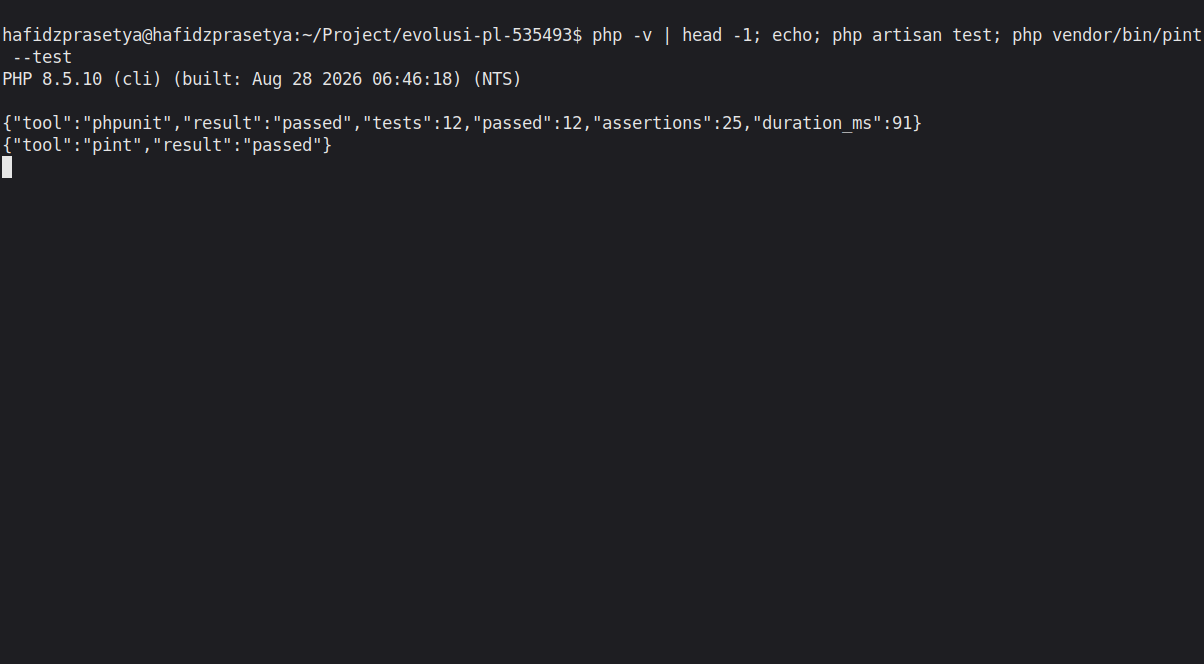
\includegraphics[width=0.95\textwidth]{images/ss-06-verifikasi-lokal.png}}
    \caption{Hasil pengujian dan pemeriksaan gaya kode di laptop.}
    \label{fig:lokal}
\end{figure}

\section{Workflow Empat Job}
Workflow \texttt{.github/workflows/ci.yml} saya perluas dari dua job menjadi empat job berurutan. Job \texttt{build} memasang dependensi dan mengunggah direktori \texttt{vendor} sebagai artefak. Job \texttt{test} mengunduh artefak itu, menyiapkan berkas \texttt{.env}, menjalankan migrasi, lalu menjalankan \texttt{php artisan test} dan pemeriksaan \texttt{pint}. Job \texttt{staging} dan \texttt{production} dirangkai dengan \texttt{needs:} setelahnya.

\begin{lstlisting}[style=yamlstyle,caption={Kerangka empat job pada \texttt{ci.yml}.}]
jobs:
  build:
    name: Build
    ...
  test:
    name: Test
    needs: build
    ...
  staging:
    name: Staging
    needs: test
    ...
  production:
    name: Production
    needs: staging
    if: github.ref == 'refs/heads/main' && github.event_name == 'push'
    environment: production
    ...
\end{lstlisting}

\subsection{Menjaga Agar Production Hanya Jalan dari \texttt{main}}
Job \texttt{production} diberi syarat \texttt{if: github.ref == 'refs/heads/main'} dan hanya bereaksi pada kejadian \texttt{push}. Karena itu, ketika kode di-push ke branch fitur, job ini dilewati walaupun job \texttt{build}, \texttt{test}, dan \texttt{staging} tetap berjalan. Saya membuktikannya dengan push ke branch \texttt{feature/pipeline-deploy}:

\begin{lstlisting}[style=bashstyle,caption={Job production terlewati pada push ke branch fitur.}]
gh run view 35198706661 --json jobs --jq '.jobs[] | "\(.name): \(.conclusion)"'
# Build: success
# Test: success
# Staging: success
# Production: skipped
\end{lstlisting}

\begin{figure}[H]
    \centering
    \customfbox{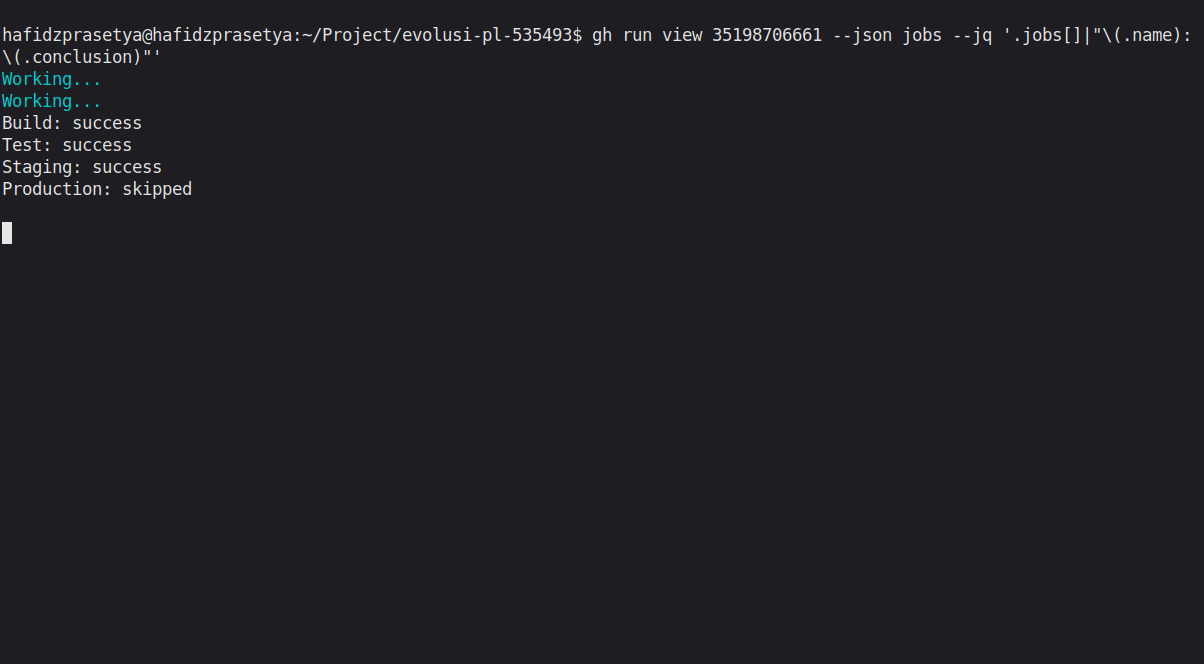
\includegraphics[width=0.95\textwidth]{images/ss-02-production-skipped.png}}
    \caption{Push ke branch fitur menjalankan build, test, dan staging, sementara production terlewati.}
    \label{fig:skipped}
\end{figure}

\subsection{Required Reviewer pada Environment Production}
Supaya deploy ke produksi menunggu persetujuan, saya membuat environment bernama \texttt{production} dan menambahkan diri sendiri sebagai \textit{required reviewer}. Verifikasi lewat API menunjukkan environment tersebut beserta reviewernya:

\begin{lstlisting}[style=bashstyle,caption={Verifikasi environment production dan reviewernya.}]
gh api repos/.../environments/production \
  --jq '{name, reviewers: [.protection_rules[].reviewers[].reviewer.login]}'
# {"name":"production","reviewers":["hafidzrizqullahprasetya"]}
\end{lstlisting}

\begin{figure}[H]
    \centering
    \customfbox{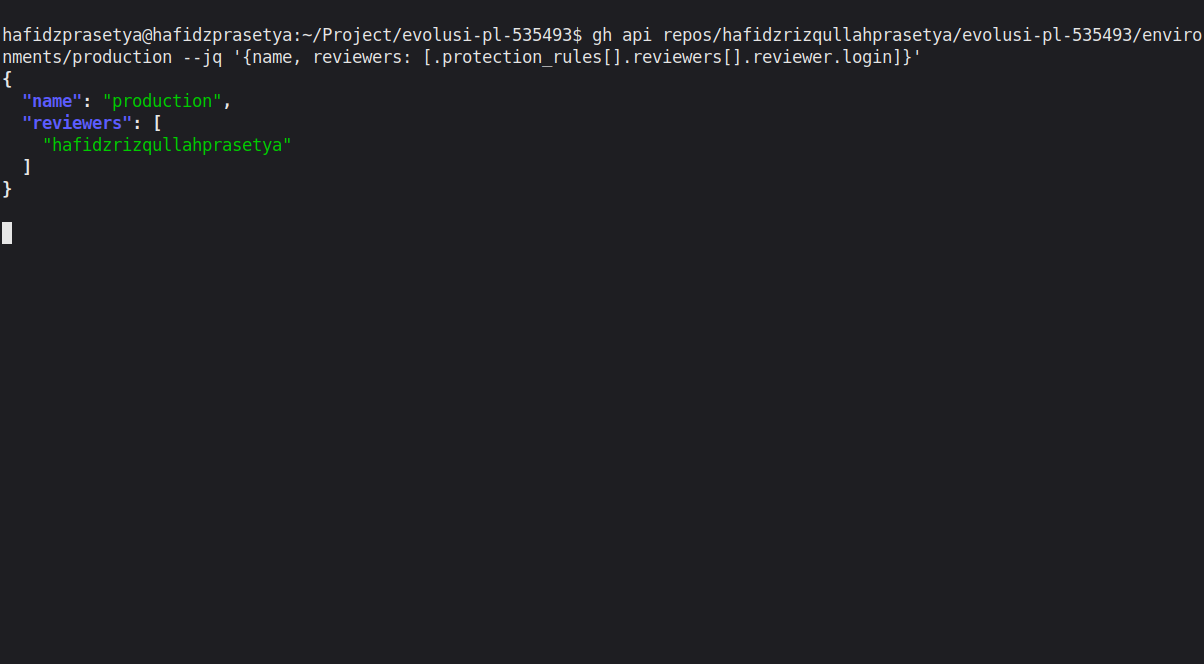
\includegraphics[width=0.95\textwidth]{images/ss-05-environment-reviewer.png}}
    \caption{Environment \texttt{production} dengan required reviewer yang terdaftar.}
    \label{fig:env}
\end{figure}

Ketika perubahan akhirnya masuk ke \texttt{main}, job \texttt{production} berhenti di status \textit{waiting} sampai saya menyetujuinya. Setelah disetujui, barulah job itu berjalan sampai selesai. Ini memperlihatkan bahwa tahap deploy benar-benar menunggu persetujuan manusia, bukan langsung jalan.

\section{Skrip Deploy di Sisi Server}
Langkah deploy di server saya tulis sebagai berkas \texttt{deploy.sh} di root repository. Isinya urutan perintah dari \texttt{artisan down} sampai \texttt{artisan up}, dengan \texttt{set -e} di baris awal agar skrip berhenti begitu ada perintah yang gagal.

\begin{lstlisting}[style=bashstyle,caption={Isi \texttt{deploy.sh}.}]
#!/usr/bin/env bash
set -e

cd /var/www/aplikasi

php artisan down --retry=60
git pull origin main
composer install --no-dev --optimize-autoloader
php artisan migrate --force
php artisan config:cache
php artisan route:cache
php artisan view:cache
php artisan queue:restart
php artisan up
\end{lstlisting}

Sesuai instruksi tugas, tahap deploy belum benar-benar dikirim ke server. Ketujuh langkah itu dituliskan sebagai \texttt{echo} di dalam job \texttt{production} supaya urutannya terlihat di log. Hasilnya tampak pada Gambar \ref{fig:log-deploy}.

\begin{figure}[H]
    \centering
    \customfbox{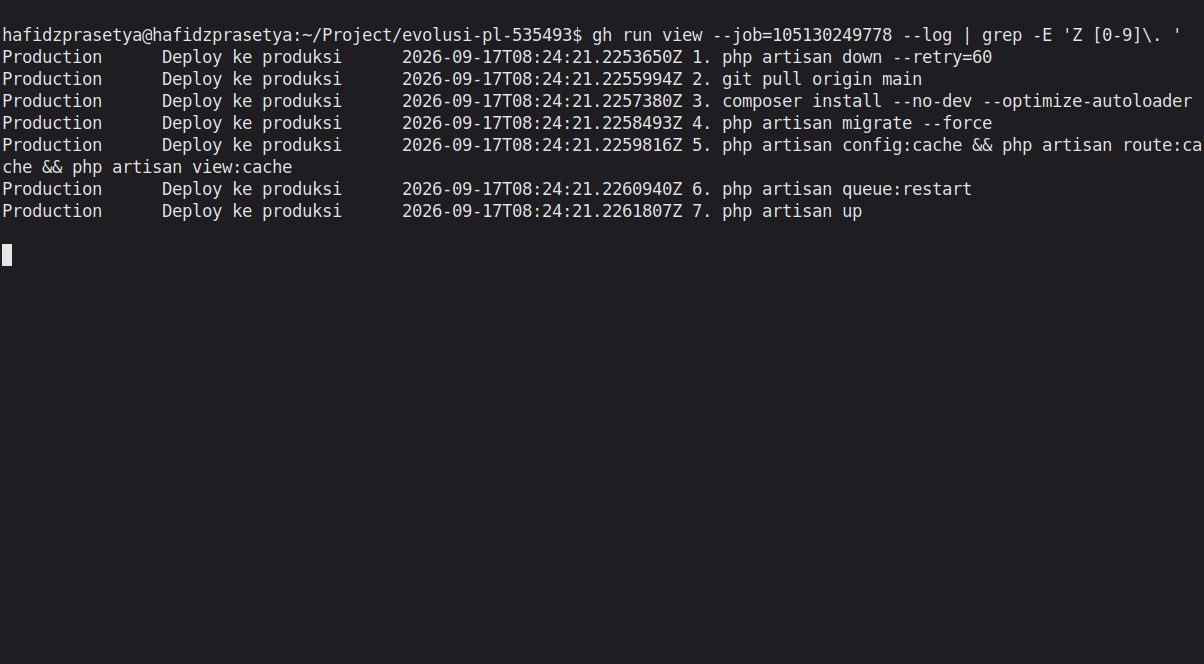
\includegraphics[width=0.95\textwidth]{images/ss-04-log-deploy.png}}
    \caption{Log job \texttt{Production} yang menampilkan ketujuh langkah deploy secara berurutan.}
    \label{fig:log-deploy}
\end{figure}

\section{Bukti Pipeline Berhenti Saat Pengujian Gagal}
Instruksi tugas meminta saya sengaja menggagalkan satu pengujian untuk membuktikan pipeline berhenti. Saya mengubah nilai harapan pada satu kasus uji di \texttt{tests/Unit/IpCalculatorTest.php} dari 3.5 menjadi 9.9, lalu push. Job \texttt{test} gagal, dan job \texttt{staging} serta \texttt{production} otomatis terlewati karena \texttt{needs:} tidak terpenuhi.

\begin{lstlisting}[style=bashstyle,caption={Pipeline merah pada satu pengujian yang sengaja digagalkan.}]
gh run view 35198536212 --json jobs --jq '.jobs[] | "\(.name): \(.conclusion)"'
# Build: success
# Test: failure
# Staging: skipped
# Production: skipped

# Failed asserting that 3.5 matches expected 9.9.
# Tests: 1 failed, 11 passed (25 assertions)
\end{lstlisting}

\begin{figure}[H]
    \centering
    \customfbox{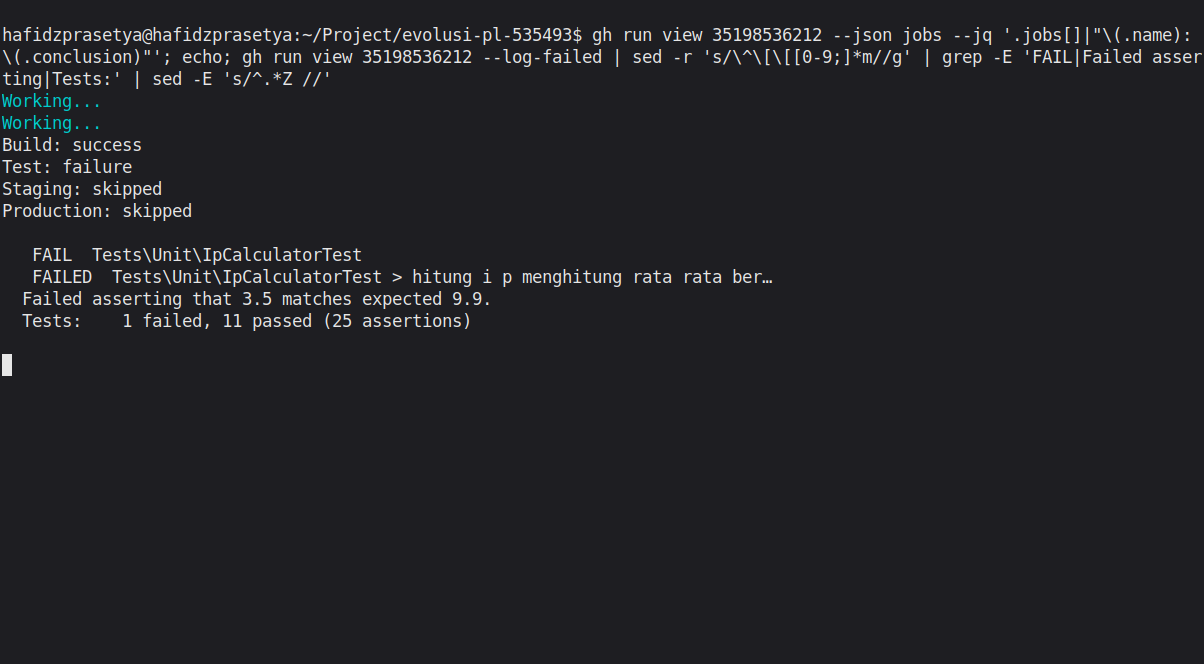
\includegraphics[width=0.95\textwidth]{images/ss-03-test-merah.png}}
    \caption{Satu pengujian yang digagalkan menghentikan pipeline: test gagal, staging dan production terlewati.}
    \label{fig:merah}
\end{figure}

Setelah bukti itu tersimpan, saya mengembalikan nilai harapan ke 3.5 dan push lagi. Pipeline kembali hijau pada commit berikutnya.

\section{Alur Pull Request dan Hasil Akhir}
Semua perubahan tetap melalui Pull Request sesuai aturan branch protection dari pertemuan pertama. Saya membuat branch \texttt{feature/pipeline-deploy} dari \texttt{dev}, membuka PR ke \texttt{dev}, lalu meneruskan \texttt{dev} ke \texttt{main}. Karena branch protection memakai status check wajib, saya juga memperbarui daftar check yang diwajibkan agar cocok dengan nama job baru (\texttt{Build} dan \texttt{Test}). Pada run terakhir di \texttt{main}, keempat job hijau:

\begin{lstlisting}[style=bashstyle,caption={Keempat job hijau pada run di branch \texttt{main}.}]
gh run view 35199310754 --json jobs --jq '.jobs[] | "\(.name): \(.conclusion)"'
# Build: success
# Test: success
# Staging: success
# Production: success
\end{lstlisting}

\begin{figure}[H]
    \centering
    \customfbox{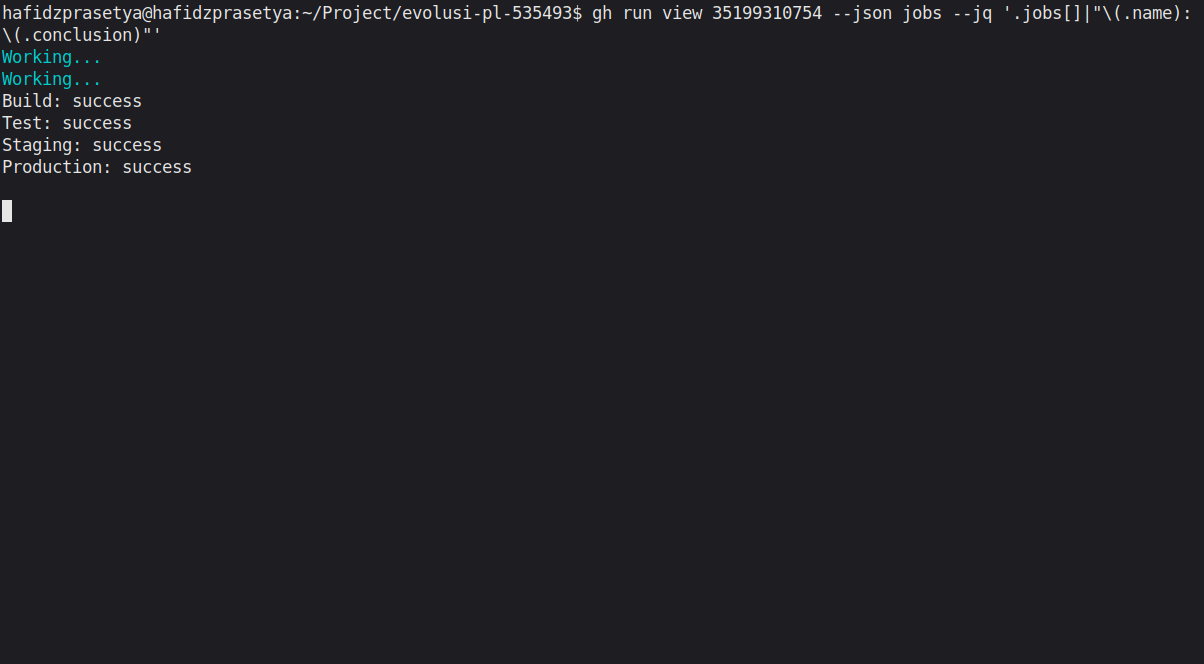
\includegraphics[width=0.95\textwidth]{images/ss-01-empat-job-hijau.png}}
    \caption{Keempat job hijau pada run di \texttt{main} setelah PR digabungkan dan deploy produksi disetujui.}
    \label{fig:hijau}
\end{figure}

\section{Kendala yang Ditemui}
Ada beberapa kendala yang saya temui. Saat direktori \texttt{vendor} dipindahkan antar job lewat artefak, izin eksekusi berkas \texttt{vendor/bin/pint} hilang, sehingga job \texttt{test} sempat gagal dengan pesan \textit{Permission denied}. Saya memperbaikinya dengan memanggil \texttt{php vendor/bin/pint} alih-alih \texttt{./vendor/bin/pint}. Mengubah nama job juga sempat menghambat karena status check wajib pada branch protection tidak lagi cocok dengan nama job yang baru, jadi daftar check perlu disesuaikan dulu sebelum PR bisa digabungkan.

\clearpage

\chapter{Kesimpulan}
Berdasarkan praktikum pada Pertemuan 3, dapat disimpulkan beberapa hal:

\begin{enumerate}
    \item Workflow berhasil diperluas menjadi empat job (\texttt{build}, \texttt{test}, \texttt{staging}, \texttt{production}) yang dirangkai dengan \texttt{needs:}, dan direktori \texttt{vendor} dipindahkan antar job lewat artefak sehingga pemasangan dependensi cukup sekali.
    \item Job \texttt{production} terbukti hanya berjalan dari branch \texttt{main}; push ke branch fitur membuat job itu terlewati sementara build, test, dan staging tetap berjalan.
    \item Environment \texttt{production} dengan required reviewer membuat deploy menunggu persetujuan manusia, dan setelah disetujui barulah job berjalan sampai selesai.
    \item Ketujuh langkah deploy Laravel dituliskan pada \texttt{deploy.sh} dengan \texttt{set -e}, lalu ditampilkan sebagai \texttt{echo} di log job \texttt{production} sesuai urutan.
    \item Pipeline terbukti berhenti ketika satu pengujian sengaja digagalkan: job \texttt{test} gagal dan job setelahnya terlewati, kemudian kembali hijau setelah kesalahan diperbaiki.
\end{enumerate}

Dengan ini pipeline repository \texttt{evolusi-pl-535493} sudah berjalan dari pengujian sampai deploy, dengan penjaga branch dan persetujuan pada tahap produksi.

\clearpage
\addcontentsline{toc}{chapter}{Daftar Pustaka}
\renewcommand{\bibname}{Daftar Pustaka}
\begin{thebibliography}{99}
    \bibitem{fowler-ci} M. Fowler, ``Continuous Integration.'' [Online]. Tersedia: \url{https://martinfowler.com/articles/continuousIntegration.html}.

    \bibitem{humble2010} J. Humble and D. Farley, \textit{Continuous Delivery: Reliable Software Releases through Build, Test, and Deployment Automation}. Addison-Wesley, 2010.

    \bibitem{github-actions} GitHub Docs, ``Understanding GitHub Actions.'' [Online]. Tersedia: \url{https://docs.github.com/en/actions/learn-github-actions/understanding-github-actions}.

    \bibitem{github-needs} GitHub Docs, ``Using jobs.'' [Online]. Tersedia: \url{https://docs.github.com/en/actions/using-jobs}.

    \bibitem{github-environments} GitHub Docs, ``Using environments for deployment.'' [Online]. Tersedia: \url{https://docs.github.com/en/actions/deployment/targeting-different-environments/using-environments-for-deployment}.

    \bibitem{github-artifacts} GitHub Docs, ``Storing and sharing data from a workflow.'' [Online]. Tersedia: \url{https://docs.github.com/en/actions/using-workflows/storing-workflow-data-as-artifacts}.

    \bibitem{laravel-docs} Laravel, ``Laravel Documentation.'' [Online]. Tersedia: \url{https://laravel.com/docs}.

    \bibitem{stauffer2023} M. Stauffer, \textit{Laravel: Up \& Running}, 3rd ed. O'Reilly Media, 2023.

    \bibitem{phpunit-docs} PHPUnit, ``PHPUnit Documentation.'' [Online]. Tersedia: \url{https://docs.phpunit.de/}.

    \bibitem{pint-docs} Laravel, ``Laravel Pint.'' [Online]. Tersedia: \url{https://laravel.com/docs/pint}.

\end{thebibliography}

\end{document}
